 \documentclass[a4paper,12pt]{article}
\usepackage[a4paper,top=1.3cm,bottom=2cm,left=1.5cm,right=1.5cm,marginparwidth=0.75cm]{geometry}
\usepackage{setspace}
\usepackage{cmap}					
\usepackage{mathtext} 				
\usepackage[T2A]{fontenc}			
\usepackage[utf8]{inputenc}			
\usepackage[english,russian]{babel}
\usepackage{multirow}
\usepackage{graphicx}
\graphicspath{ {./images/} }
\usepackage{wrapfig}
\usepackage{tabularx}
\usepackage{float}
\usepackage{longtable}
\usepackage{hyperref}
\hypersetup{colorlinks=true,urlcolor=blue}
\usepackage[rgb]{xcolor}
\usepackage{amsmath,amsfonts,amssymb,amsthm,mathtools} 
\usepackage{icomma} 
\mathtoolsset{showonlyrefs=true}
\usepackage{euscript}
\usepackage{mathrsfs}

\DeclareMathOperator{\sgn}{\mathop{sgn}}
\newcommand*{\hm}[1]{#1\nobreak\discretionary{}
	{\hbox{$\mathsurround=0pt #1$}}{}}


\title{\textbf{Определение скорости полета пули при помощи баллистического маятника (1.2.1)}}
\author{Павлушкин Вячеслав}
\date{December 2021}


\begin{document}
	
	\maketitle
	
	\section{Введение}
	
	\textbf{Цель работы:}
	Определить скорость полёта пули применяя законы сохранения и использую баллистические маятники
	
	\noindent\textbf{Оборудование:}
	Духовое ружьё на штативе, осветитель, оптическая система для измерения отклонений маятника, измерительная линейка, пули и весы для их взвешивания, баллистические маятники.
	\section{Ход работы}
	
	\subsection{Метод баллистического маятника, совершающего поступательное движение}
	В этой части работы будем использовать установку, изображённую на рисунке ниже. При попадании пули в цилиндр любая его точка движется по окружности известного радиуса, поэтому его смещение с помощью собирающей линзы можно перевести в линейное отклонение на линейке.
	
	\begin{figure}[H]
		\begin{center}
			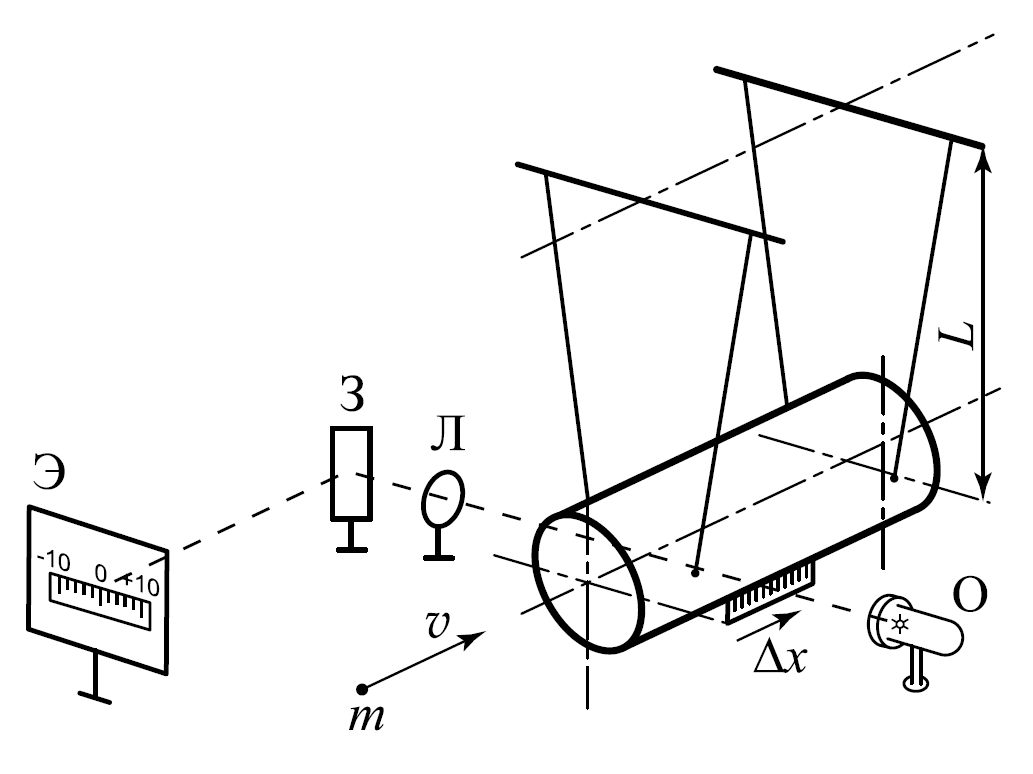
\includegraphics[scale = 0.56]{1.2.1 ustan1}
			\caption{схема установки для измерения скорости полета пули}
		\end{center}
	\end{figure}
	
	При контакте пули с цилиндром можно записать ЗСИ:
	\begin{equation}
		 mu = (M+m)V
	\end{equation}
	где $m$ -- масса пули, $u$ -- скорость пули перед ударом, $V$-скорость цилиндра вместе с пулей после удара.
	\begin{equation}
		u=\frac{M+m}{m}V \approx \frac{M}{m}V \;\;\;\;\; V^2=2gh \;\;\;\;\; h = L(1-cos \varphi ) = 2L^2 sin \frac{\varphi^2}{2} \;\;\;\;\;\;\; \varphi \approx \frac{\Delta x}{L} 
	\end{equation}
	Тогда скорость пули можно выразить как
	\begin{equation} \label{vel1}
	 u=\frac{M}{m} \sqrt{\frac{g}{L}} \Delta x
	\end{equation}

	При измерении было замечено, что за 10 периодов амплитуда колебаний почти не уменьшилась, поэтому их затуханием можно пренебречь.
	
	Для начала проверим работоспособность установки, а именно проведем несколько холостых выстрелов по маятнику и убедимся в том, что он практически не реагирует на удар воздушной струи.
	
	Вычислять скорость пули будем по форуле \eqref{vel1}, для чего нужно проверить, что за 10 колебаний амплитуда уменьшалается меньше, чем на половину.
	
	Произведем 4 выстрела, запишем амплитуды, полученные при выстрелах, и по их значениям найдем скорости пуль.
	
	\begin{table}[H]
		\begin{center}
			\begin{tabular}[H]{|c|c|c|c|c|}
				\hline
				$m$, г & 0,504 & 0,508 & 0,506 & 0,502\\ \hline
				$\Delta x$, мм & 12,75 & 13,75 & 13,5 & 13,5\\ \hline
				$u$, м/с & 156,1 & 165 &164,6 &170 \\ \hline
			\end{tabular}
		\caption{}
		\end{center}
	\end{table}
	
	\noindent наша установка имела параметры: $M = (2925 \pm 5)$ г, и $L = (220,4 \pm 0,1)$ см.

	Средняя скорость пули \underline{$u_\text{ср} = 163,9$ м/с}, а погрешность будет равна:
	
	\begin{equation}
		\sigma_u^{\text{сист}} =u \sqrt{\varepsilon_M^2 + \varepsilon_m^2 + \varepsilon_{\Delta x}^2 + \left(\frac{\varepsilon_L}{2} \right)^2}  \;\;\;\;\; \sigma_u^{\text{случ}} = \sqrt{ \frac{1}{n(n-1)} \sum_{i=1}^{n}(u_i - u_{\text{ср}})^2} \;\;\;\;\; \sigma_u =\sqrt{\sigma_{\text{сист}}^2 + \sigma_\text{случ}^2} 
	\end{equation}
	\begin{equation}
		\sigma_u^\text{сист}\approx 3,1 \text{ }\dfrac{\text{м}}{\text{с}} \;\;\;\;\;\;\;\;\;\;\;\;\;\;\;\;\;\;\;\;\;\;\;\;\;\;\;\;\;\;\; \sigma_u^\text{случ}\approx 2,9 \text{ }\dfrac{\text{м}}{\text{с}} \;\;\;\;\;\;\;\;\;\;\;\;\;\;\;\;\;\;\;\;\;\;\;\;\;\;\;\;\;\;\;
		\sigma_u \approx 4,2 \text{ }\dfrac{\text{м}}{\text{с}}
	\end{equation}
	
	Окончательно получаем скорость пули равную \underline{$u = (163,9 \pm 4,2)\text{, }\dfrac{\text{м}}{\text{с}}$}
	
	\subsection{Метод крутильного баллистического маятника}
	
	В этой части работы мы будем использовать крутильный баллистический маятник. Схема установки представлена на картинке ниже.
	
	\begin{figure}[h]
		\begin{center}
			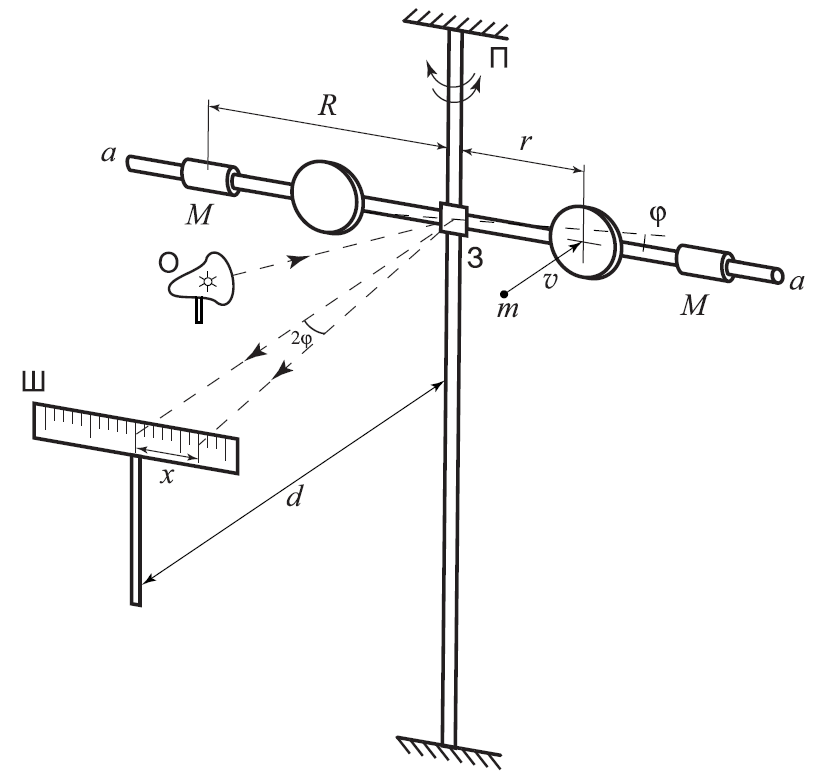
\includegraphics[scale = 0.66]{1.2.1 ustan2}
			\caption{схема установки для измерения скорости полета пули с баллистическим маятником}
		\end{center}
	\end{figure}
	
	Считая удар неупругим, можно записать уравнение
	$$mur=I \Omega$$
	$r-$расстояние от линии полёта пули до оси вращения, $I$ -- момент инерции относительно этой оси, $\Omega$ -- угловая скорость маятника сразу после удара.
	
	Можно пренебречь затуханием колебаний и потерями энергии и записать ЗСЭ:
	$$ k \frac{\varphi^2}{2} = I \frac{\Omega^2}{2} $$
	\noindent где $k$ -- модуль кручения проволоки, $\varphi$ -- максимальный угол поворота маятника, тогда:
	\begin{equation} \label{vel2}
		 u = \varphi \frac{\sqrt{kI}}{mr} 
	\end{equation}
	Измерим растояние от оси вращения до штатива с линейкой $d = 59,3 \pm 0,1 \text{ см}$, тогда в силу малости колебаний можно найти $\varphi$ как
	
	\begin{equation}
		\label{phi}
		\varphi \approx \frac{x}{2d}
	\end{equation}
	
	где $x$ -- смещение изображения нити осветителя на шкале, которое легко можно измерить.
	
	Периоды колебаний маятника с грузами и без можно выразить как
	$$T_1= 2 \pi \sqrt{\frac{I - 2MR^2}{k}} \;\;\;\;\;\; T_2 = 2 \pi \sqrt{\frac{I}{k}}$$
	Тогда $\sqrt{kI}$ можно найти как:
	\begin{equation}
		\sqrt{kI} = \frac{4 \pi M R^2 T_2}{T_2^2 - T_1^2}
		\label{kl}
	\end{equation}
	$R$ -- расстояние от оси вращения до центров грузиков, $M$ - масса грузиков.
	
	Для начала запишем данные установки: $ r = 22 \text{ см} \text{, } R = 33,6 \text{ см} \text{, } M_1 = 729,9\text{ г} \text{, а } M_2 = 729,6 \text{ г} $.
	
	Снимем периоды колебаний после выстрела с грузиками и без, чтобы найти $\sqrt{kI}$:
	
	\begin{table}[H]
		\begin{center}
			\begin{tabular}{|c|c|c|c|}
				\hline
				№  & $t$, с  & $T$, с&  N \\
				\hline
				1. С грузами & 155,94& 15,594 & 10\\
				\hline
				2. С грузами & 151,79 & 15,179& 10\\
				\hline
				3. Без грузиков & 199,28 & 19,928& 10\\
				\hline
				4. Без грузиков & 199,64 & 19,964& 10\\
				\hline  
			\end{tabular}
			\caption{Периоды колебаний баллистического маятника после выстрела}
		\end{center}
	\end{table}

	Из таблицы получаем, что $T_1^{\text{ср}} = (15,387 \pm 0,207) \text{ см}$, а $T_2^{\text{ср}} = (19,946 \pm 0,03)\text{ см}$. С помощью полученных периодов колебаний найдем $\sqrt{kI}$ по формуле \eqref{kl}:
	
	$$\sqrt{kI} \approx 138,18 \cdot 10^{-3} \text{ } \dfrac{\text{кг}\cdot\text{м}^2}{\text{c}} \;\;\;\;\;\; \sigma_{\sqrt{kI}} = \sqrt{kI} \cdot \sqrt{\varepsilon_{T_2^2-T_1^2}^2 + \left(2\varepsilon_{R^2}\right)^2 + \varepsilon_M^2 + \varepsilon_{T^2}^2} \approx 0,54 \cdot 10^{-3} \text{ } \dfrac{\text{кг}\cdot\text{м}^2}{\text{c}}$$
	
	Теперь по формулам \eqref{vel2} и \eqref{phi} определим $\varphi$ и скорость пули. Получаем таблицу:

	\begin{table}[!h]
		\begin{center}
			\begin{tabular}{|c|c|c|c|c|}
				\hline
				& $m$, г& $x$, cм&  $\varphi$, рад& $u$, м/с\\
				\hline
				без грузиков & 0,514 & 15,75 &0,13 & 162,28\\
				\hline
				без грузиков &0,510 &14,50  & 0,12 & 150,57 \\
				\hline
				с грузиками & 0,507 &16,10  &0,14  &168,17  \\
				\hline
				с грузиками & 0,517 &15,50  & 0,13 & 158,77\\
				\hline 
			\end{tabular}
			\caption{Таблица полученных скоростей}
		\end{center}
	\end{table}
	\begin{equation}
		\sigma_u^{\text{сист}} = u\cdot \sqrt{ \varepsilon_x^2+ \varepsilon_d^2+ \varepsilon_{\sqrt{kI}}^2 + \varepsilon_m^2 + \varepsilon_r^2 } \;\;\;\;\;\; \sigma_u^{\text{случ}} =  \sqrt{\frac{1}{n(n-1)} \sum_{i=1}^{n}(u_i - \overline{u})^2} \;\;\;\;\;\;
		\sigma_u = \sqrt{\sigma_{\text{случ}}^2 + \sigma_\text{сист}^2}
	\end{equation}
	
	Тогда средняя скорость \underline{$u_\text{ср} = (159,95 \pm 1,44)\text{ }\frac{\text{м}}{\text{с}} $}
	
	\section{Вывод}
	
	\indent Были полученны скорости пули двумя методами:  методом баллистического маятника, совершающего поступательное движение, и методом крутильного баллистического маятника. Разброс полученных значений связан как с ошибками опыта, так и с различием скоростей пуль от выстрела к выстрелу. Так же имеет значение то, что стрельба в каждом методе производилась своим ружьем.
	
\end{document}